%\chapter{models}\label{sec:expansion}
\section{Halo Expansion}\label{sec:expansion}

Explanation of the Method..


\begin{equation}
\rho = \sum \sum \sum
\end{equation}

\subsection{Isolated MW halo expansion}

Fig.1 MW scatter plot with color code the potential,

\begin{figure}[H]
\centering
\includegraphics[scale=0.5]{../code/Snlm_MW.png}
\end{figure}

\begin{figure}[H]
\centering
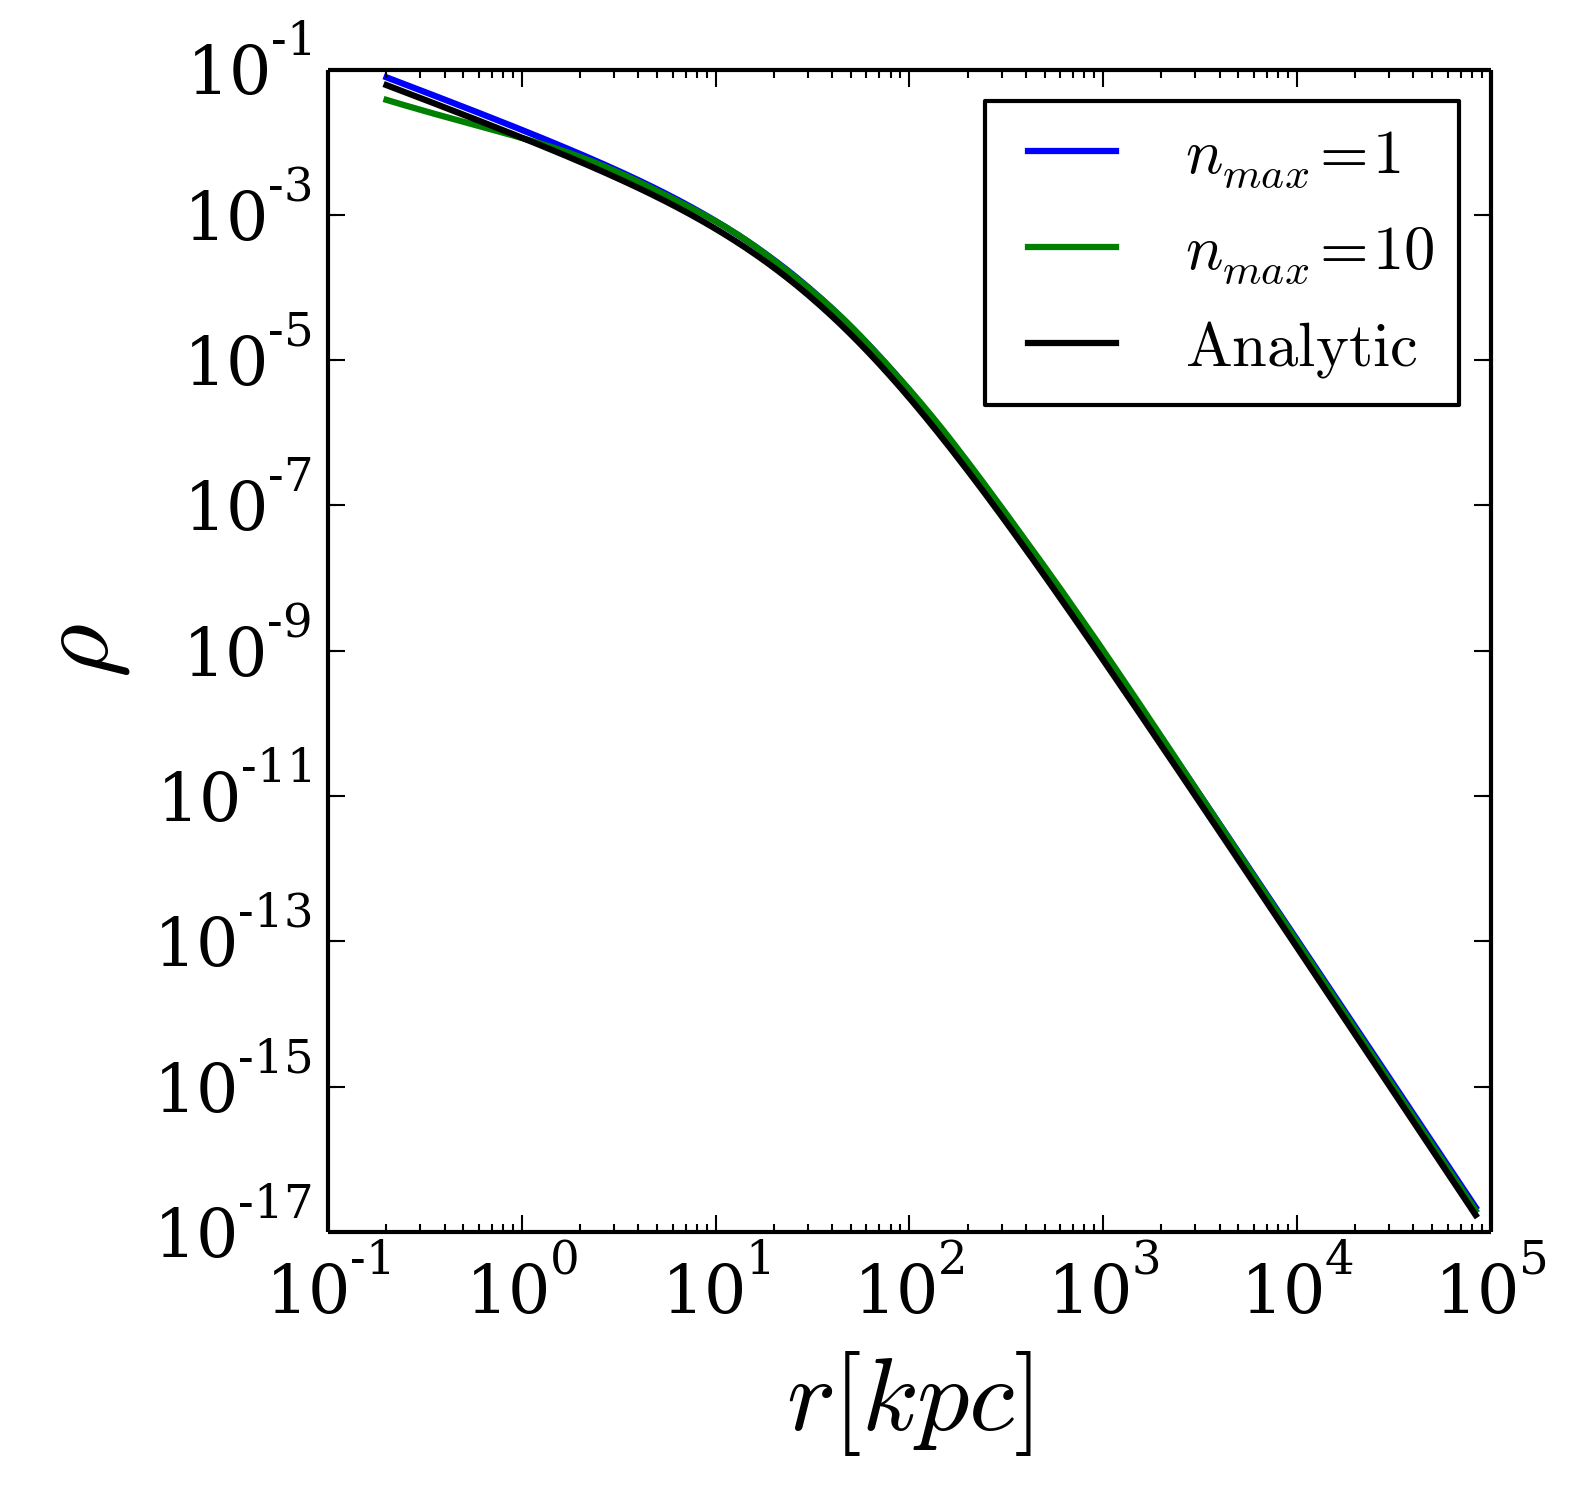
\includegraphics[scale=0.5]{../code/rho_MW.png}
\includegraphics[scale=0.5]{../code/pot_MW.png}
\end{figure}

\begin{figure}[H]
\centering
\includegraphics[scale=0.5]{../code/2dpot_MW.png}
\end{figure}


\begin{figure}[H]
\centering
\includegraphics[scale=0.5]{../code/2dpot_ratio_MW.png}
\end{figure}


\begin{figure}[H]
\centering
\includegraphics[scale=0.5]{../code/2dpot_res_MW.png}
\end{figure}



\begin{figure}[H]
\centering
\includegraphics[scale=0.5]{../code/MW_orbits_biffn1.png}
\end{figure}


\begin{figure}[H]
\centering
\includegraphics[scale=0.5]{../code/MW_orbits_biffn1n10.png}
\end{figure}


\begin{figure}[H]
\centering
\includegraphics[scale=0.5]{../code/MWyz_orbits_biffn1n10.png}
\end{figure} 


\subsection{LMC + MW}


\begin{figure}[H]
\centering
\includegraphics[scale=0.5]{../code/MWLMC_xy_orbits_biffn20n20.png}
\end{figure}


\begin{figure}[H]
\centering
\includegraphics[scale=0.5]{../code/MWLMC_yz_orbits_biffn20n20.png}
\end{figure}

 
\subsection{LMC + MW evolving in time}

\begin{figure}[H]
\centering
\includegraphics[scale=0.5]{../code/MWLMCt_xy_orbits_biffn20n20.png}
\end{figure}


\begin{figure}[H]
\centering
\includegraphics[scale=0.5]{../code/MWLMCt_yz_orbits_biffn20n20.png}
\end{figure}


